\documentclass[prb,twocolumn]{revtex4-2}
\usepackage{graphicx}
\usepackage{amsmath}
\usepackage{amssymb}
\usepackage{epstopdf}

\begin{document}
\title{Assignment 5}

\author{James Lawton}
\affiliation {
Physics Department, Virginia Tech, Blacksburg, Virginia 24061, USA\\
}


\begin{abstract}
Abstract: Here we are looking to analyze and simulate the behaviors of a circuit and atomic structures
\end{abstract}

\maketitle

\section{Problem 5-1}

\noindent
Here we look to find the currents in an unbalanced Wheatstone bridge with the following properties:
$r_1 = r_2 = 100 \Omega$, $r_3 = 150 \Omega$, $r_x = 120 \Omega$, $r_a = 1000 \Omega$, and $r_s = 10 \Omega$.

\begin{figure}[h!]
\centerline{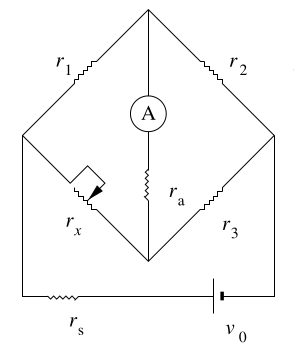
\includegraphics [width=3 in] {circuit}} \caption{Circuit Diagram} \label{secant}
\end{figure}

Utilizing Gaussian Elimination with partial pivoting, we can find and plot our findings with various values for $v_0$. We solve the following matrix equation for $x$ where $x$ contains the currents.

\begin{eqnarray}
  Ax = b \\
  A =
  \begin{bmatrix}
    10 & 100 & 100 \\
    -120 & 1220 & -1000 \\
    -150 & -1000 & 1250
  \end{bmatrix},\ \ \ \ 
  b = 
  \begin{bmatrix}
    v_0 \\
    0 \\
    0
  \end{bmatrix}, 
  \label{namefornewequation}
\end{eqnarray}

The simulation was run with $v0$ ranging from $0$ to $100$. The results plotted  obtained over:

\begin{figure}[h!]
\centerline{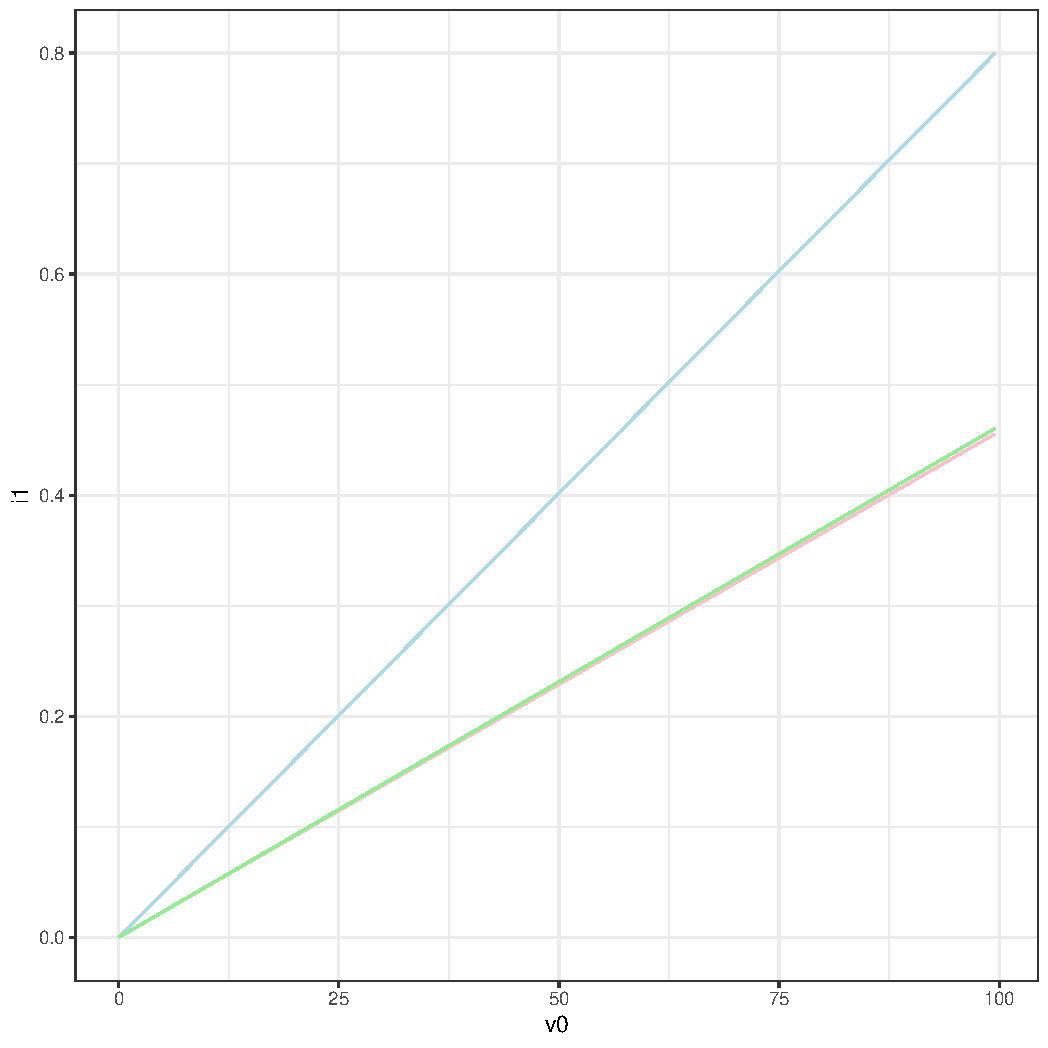
\includegraphics [width=3 in] {5-1}} \caption{Secant Method} \label{secant}
\end{figure}

Here we can see that the three currents increase linearly with the voltage. 

\section{Problem 5-5}

Here we look to find a stable geometric structure for clusters of Na+ and Cl- ions by using the Secant method to solve the following equation:

\begin{eqnarray}
V(r_{ij})=\eta_{ij}\frac{e^2}{4\pi\epsilon r_{ij}}+\delta_{ij}V_0e^{-r_{ij}/r_0} \\
  U(r_1, r_2, ... r_n) = \sum_{i>j}^{n}{V(r_{ij})}
\label{namefornewequation}
\end{eqnarray}

The goal here is to minimize the second equation. We do this by finding where the slope is zero which indicates that there is a stable geometric structure.

\begin{thebibliography}{99}

\bibitem{thecoursetext} T. Pang, \emph{Introduction to Computational Physics}, Cambridge University Press (2006).

\end{thebibliography}

\end{document}
